\documentclass[compsoc]{IEEEtran}
% \documentclass[conference,compsoc,twoside]{IEEEtran}
\usepackage[utf8]{inputenc}
\usepackage{hyperref}
\usepackage{natbib}
\usepackage{graphicx}
\usepackage{wrapfig}
\usepackage{lscape}
\usepackage{rotating}
\usepackage{epstopdf}
\usepackage{xparse}

% \makeatletter
% \DeclareDocumentEnvironment{appendixfig}{}{
%   \par\medskip\noindent
%   \begin{minipage}{\linewidth}{
%   \def\@captype{figure}
%   \centering
% }
% \end{minipage}{
% \par\bigskip
% }}
% \makeatother 

\title{Intelligent Agents in Real-Time Strategy Games}

\author{
    \IEEEauthorblockN{
        M. Bakirci,
        J. Mulder, 
        M. Dias Avelino,
        P. Popieluch,
        T. Schijvenaars and
        A. Wali
    }

    \IEEEauthorblockA{
        Faculty of Electrical Engineering, Mathematics and Computer Science,
        TU Delft\\
        Delft, The Netherlands\\
        \{
            m.bakirci, 
            j.mulder-5, 
            m.diasavelino, 
            p.popieluch, 
            t.c.f.schijvenaars, 
            a.wali-1
        \}@student.tudelft.nl
    }
}

\date{February 2019}

\begin{document}

\maketitle

\begin{abstract}
Real-time strategy games have been proven to be a perfect environment in which to study artificial intelligence techniques. This lead to a large increase of research being done on different topics within the scope of real-time strategy games, which makes it very difficult to have a general overview of all the progress made. This paper summarizes the most notable and state-of-the-art artificial intelligence techniques that have been applied to specific areas of real-time strategy games in the past couple of years. 


% The most notable game was StarCraft for which ..... ! hier een stukje over alle research papers betreffende StarCraft ! ..... While a lot of techniques seem really promising, most of them still have a long way to go to deliver human-level performance.
\end{abstract}


% Marcelo
\section{Introduction}
\IEEEPARstart{F}{or} the past fifteen years since Buro's\citep{buro2004call} call for more AI research in the Real-Time Strategy (RTS) game genre, the field has made impressive progress. It has grown from the simple AI shipped with games in single-player campaigns or bots to play skirmishes against to the milestones of DeepMind's AlphaStar\citep{arulkumaran2019alphastar} or OpenAI's Five\citep{openaifive} winning against professional players. 

This progress has been stimulated by the well-defined environments provided by RTS games whose difficulty can be tailored for specific aspects of AI training and complexity is reminiscent of real life scenarios. In his motivation for RTS AI research\citep{buro2004rts}, Buro defines multiple fundamental research problems:
\begin{itemize}
    \item Decision making under uncertainty
    \item Spatial and temporal reasoning
    \item Adversarial real-time planning
    \item Opponent modelling/learning
    \item Resource management
    \item Collaboration
\end{itemize}

Each of these problems can and have been tackled in unique ways with various degrees of success using both algorithms developed in different fields. For example Influence Maps\citep{uriarte2012kiting} that were originally developed for robot navigation and have now been used for micromanaging units in an RTS game, or Deep Learning\citep{lecun2015deep} and Reinforcement Learning\citep{mnih2015human} which were developed specifically for AI and enable the bot to analyze what it sees and learn from its experiences.

Being able to approach these challenges in so many different ways makes it a daunting and difficult task to keep track of the fast, if not sometimes exponential, progress of the field of AI. This survey aims to provide a glimpse into some of the current state-of-the-art methods and algorithms applied to the genre of RTS.

\subsection{Background of RTS games}
Real-Time strategy games are a sub-category of strategy games but where the game progresses in real time, meaning the game is not divided into ordered turns and each player can play at his own pace. This in contrast to, for example, a game like Civilization\citep{civilization}.

RTS games are usually war games where multiple players start in different places in a game map without any knowledge of where their opponents are located and no resources readily available to them. The goal of the game is to collect resources from the environment use those resources to upgrade their base and build-up an army to ultimately defeat their opponents, and in the end being the last one standing. These games often contain multiple factions a player can choose from, with each having their own strengths, weaknesses and optimal ways of playing them.

These games combine multiple difficult scenarios and challenges as the game progresses. A good player needs to be able to control its unit in a fast and precise way, known as \textit{micromanaging}, with professional players being able to reach 400 actions per minute\citep{apmwcs}. A strong micromanagement allows the player to gather more information on the adversary through scouting, to harass the enemy's base and disrupting his economy, and can change the tide of battle by being able to deal more damage to the opponent's units while taking less damage by using techniques such as \textit{kiting}. Kiting consists of dealing damage to an enemy while keeping enough distance that the enemy is not able to deal damage back. An AI needs therefore needs to learn how to control units and come up with strategies on how to use and combine all different types of units, with all their advantages and disadvantages.

The flip side of micromanagement is called \textit{macromanagement}. This is the ability to come up with a strategy on how to setup the resource economy and what to spend it on, often referred to as planning. Resources are scarce and its gathering is very slow at the beginning, making it very important to devise an optimal plan on what to spend it on because a wrong decision can impair the economic momentum and therefore widening the progress gap between players.

For example, at the beginning the player has to devise the most efficient way to gather resources and which building and/or units should be prioritized, a strategy which is very dependant on the faction selection of the opponent(s), which translate different possible strategies being used. For example, the other player(s) might choose to attack very early on catching the player unaware and unprepared because the player was focusing on increasing resource production instead of building defenses. On the other hand, if the player spends too many resources building defenses early in the game it might impair the development of the player's economy, allowing the opponent(s) to build stronger units first and as such making the player's earlier built defenses obsolete.

Some examples of these types of games are Blizzard's StarCraft\citep{starcraftgame} or WarCraft\citep{warcraftgame}, which are RTS games that take place in the future or in a fantasy world respectively, and Ensemble Studios' Age of Empires\citep{ageofempiresgame}, which is a game based on historical events and factions.

The many strategies and considerations an AI algorithms has to take into account, many of which are yet to be discovered or will be made obsolete when a new update to the game is released, means RTS games provide a difficult, complex and good benchmark.

% Van hier
\subsection{Research Question and Sub-questions}

The initial goal of this literature review was to summarize the state of the art and open challenges within the field of RTS for AI. Because the problems presented in the beginning of this chapter cover a very broad and disparate area of research, a selection of papers with promising techniques was made. Each paper covers one or multiple research problems (e.g. Adversarial Real–time Planning, Opponent Learning, and Spatial and Temporal Reasoning) and answer the following research question:

\vspace{2mm}
\textit{"What AI techniques and algorithms have been used to solve some of the fundamental research problems in RTS games?"}
\vspace{2mm}


To better answer the main research question, sub-questions were made:
\begin{description}
\item[\textit{"How does the technique work?"}]
\item[\textit{"What are the strong and weak points of the technique?"}]
\end{description}

The first sub-question is specified to give the reader a notion on how the technique works and what applications it has. The second sub-question is meant to give the reader an idea on how effective this technique can be when used for its specific task.

\subsection{Outline}

The paper will be structured in the following order:
% Tot hier

Chapter \ref{chapter:macro-management} will go into detail on how the macro-management component of a bot can be trained purely by learning from game replays and used for Adversarial Real–time Planning.

Chapter \ref{chapter:genetic-building} explains how an genetic algorithm can be used to determine the most optimal building placement strategy to deter enemy assaults.

Chapter \ref{chapter:generalizing-planning} falls within the Opponent Learning category and describes how Reinforcement Learning can be applied for the micro-management of units during combat.

Chapter \ref{chapter:starcraftmultiagentchallenge} \& \ref{chapter:alphastar} summarize the accomplishments of StarCraft bots when pitted either against each other or against real players.

% Appendix "something" is a mindmap which gives a general overview of what algorithms have been used to solve certain research problems in RTS games.


% Tim
\section[Learning Macromanagement]{Learning Macromanagement\citep{justesen2017learning}} 
\label{chapter:macro-management}

\subsection{About}
All tasks related to planning and strategy are called macromanagement. This section discusses the findings of a research paper about the training of a neural network in macro management of StarCraft. The research presented a way to train a neural network which predicts macromanagement actions based on replays, which were live-action replays of expert human StarCraft players. Learning based on human actions can be described as imitation learning and the technique that is used by the authors of the paper, predicts actions based on games that are played by human players. Finally, the trained neural network has been put to action by applying it to an existing StarCraft bot: the UAlbertaBot. The UAlbertaBot is an open source, modular StarCraft bot\citep{churchill2015ualbertabot}. The modularity of the UAlbertaBot refers to the multiple agents within the bot with different tasks (e.g. macro management, micromanagement and pathfinding). These dedicated modules can be developed by anyone\citep{ontanon2013survey}. The module of the UAlbertaBot that will be swapped with the trained neural network is called the production manager. The production manager regulates the build order of troops and upgrades.

\subsection{Applied Methods and Techniques}

The neural network that is going to replace the standard production manager is trained based on the live-action replays. The training data consists of 2005 different matches between the Protoss and Terran race in StarCraft. From these matches, the following events were extracted: when units, upgrades or buildings are produced, when units or buildings are destroyed and when enemy units and buildings are observed. These events are used to simulate abstract StarCraft games via the build order forward model presented in Justesen and Risi\citep{justesen2017continual}. A build order forward model is a model which simulates the outcome of a build order, based on the current unit composition and available information about the opponent. The model is a predecessor of the macromanagement model which is presented in this paper, and favors short-term rewards over long-term rewards. The match-data is converted into state-action pairs by the StarCraft game engine, which resulted in a data set of 789,571 of such pairs. These were split up between a training set and a test set, in an 80:20 ratio respectively.

The neural network itself is a simple multi-layered network architecture with fully-connected layers. The problem is treated as a classification problem, in which the network tries to predict the next build given a game state. The output of the network is thus the probability of producing each build in a given state. The network is trained on the training set which is shuffled before each epoch. Xavier initialization is used for all weights in the hidden layers and biases are initialized to zero. Xavier initialization is an initialization process to assign network weights in such a way that the variance remains the same for a linear neuron\citep{glorot2010understanding}.
\begin{equation} \label{eq:xav}
y_i = x_iw_i + b_i
\end{equation}
The activation function of such an initialization is shown in equation (\ref{eq:xav}). In this equation $y_i$ is the argument vector, $x_i$ the activation vector and $w_i$ the weight at layer $i$.
Also, the learning rate is 0.0001 with the Adam optimization algorithm and a batch size of 100. The Adam optimization algorithm is an extension to stochastic gradient descent, which is used to update the network weights\citep{kingma2014adam}.

After training, the neural network is then applied to the UAlbertaBot instead of the standard production manager. The performance of the bot is split into two policies: greedy action and probabilistic action. The greedy action policy always selects the build with the highest probability. The probabilistic action policy selects builds with the probabilities of the softmax output units. The performance of the bot was tested in multiple 1 versus 1 - Protoss versus Terran - matches versus different in-game bots. The probabilistic action policy achieved a 59\% win rate against the built-in StarCraft bot when blind and a 68\% win rate when also receiving information about the opponent's material. The greedy strategy achieved a win rate of 53\% against the built-in bot. However, the neural network lost 100\% of all games played versus a bot with an powerful hand-designed rush strategy.

\subsection{Contributions to Reinforcement Learning}

According to Justesen and Risi\citep{justesen2017learning}, deep learning has never been used before to train a neural network to learn a specific function like macro management in a larger AI architecture. It is shown that macromanagement tasks can be learned from replays using deep learning, and that the learned policy can be used to outperform the built-in bot in StarCraft. The results were promising, but it did not lead to a bot that was able to deliver performance on-par with that of a human player.

One of the advantages is that by using state-action pairs, you can speed up the training enormously, since you can train the neural network on specific areas of interest. A problem with learning from replays, is that performance mostly depends on the quality of replays. A bot that is trained with imitation learning can never exceed the level of play displayed in the training set. It does not learn how to improve beyond that point.

\subsection{Future plans}

Further research would implement the trained neural network to a more sophisticated modular StarCraft bot that is capable of controlling multiple bases and more advanced units. Another plan for the future would be extending the current approach by applying regularization techniques (adding information to reduce overfitting) and including positional information of units and buildings. With these adjustments, the final plan for the future would be to improve this bot to compete with other high-performing StarCraft bots. 

% Piotr
\section[Building Placement Optimization]{Building Placement Optimization\citep{barriga2014building}}
\label{chapter:genetic-building}

\subsection{About}

One of the sub-problems of RTS games is the problem of Building Placement, which can be classified as a spatial and temporal reasoning problem as defined by Buro. This problem is concerned with constructing buildings at strategic locations with the goal of slowing down potential enemy attacks as much as possible while still allowing friendly units to move around freely. Strategic building placement is crucial for top-level play in RTS games\citep{barriga2014building}.

Building placement is a complex combinatorial optimization problem which cannot be solved by exhaustive enumeration on today’s computers\citep{barriga2014building}. Traditionally, RTS game bots used several less sophisticated techniques which depend on hard-coded domain rules, map analysis libraries and simple spiral search. This paper investigates the use of a Genetic Algorithms (GA) to solve the problem.

\subsection{Applied Methods and Techniques}

GAs are search algorithms which can be used to solve combinatorial optimization problems. The working of GAs is inspired by Darwin's evolution theory\citep{darwin1859origin}. The researchers chose to use a GA because the place of buildings can be easily represented in a chromosome.

In a GA we start with a pool of randomly generated chromosomes. A chromosome represents a solution to the problem and consists of genes, each gene represents a variable. In this implementation a gene represents a building and contains the buildings position on the game map. The order of genes is maintained, every gene (position) represents a specific building.

For each chromosome the fitness is determined by simulating a game from a battle specification. The battle specifications are based on replays from top human players and bots. The fitness score is the value of the remaining army after a battle ended. The value of the army is the sum of the values of the remaining units, the value of the units is calculated by rules based on the mineral cost, gas cost, health and the type of the unit. The value is negative when the battle is lost.

After the fitness is determined, chromosomes need to be selected for reproduction. Selection happens by the roulette wheel selection process\citep{goldberg89} with linear scaling of the fitness. Every chromosome has a slot in a roulette wheel where the size of the slot is determined by the fitness. A higher fitness results in a larger slot which increases the probability that this specific chromosomes will be selected. Selected chromosomes are copied to a mating pool.

Now, the chromosomes in the mating pool are randomly paired. Each pair of chromosomes undergoes a crossover and produces two children. The researches have chosen to use uniform crossover instead of the more traditional N-point crossover because they believe that there is little relationship between two genes (location of two buildings). In uniform crossover, every child's gene is selected randomly from one of the two parents' genes from the same gene position.       

For each gene in a child's chromosome a mutation operator can be executed. The mutation operator moves the building randomly near by its current location. Whether the operator is executed is determined randomly with a small probability.

As a consequence of the random selection of the chromosomes it could occur that the best performing chromosome is not selected for mating. This could result in that the best found solution will be lost. To prevent this from happening a process known as elitism is applied. With elitism, the chromosome with the highest fitness is copied unaltered to the new chromosome pool, no cross-over or mutation is applied.

At some point the algorithm needs to terminate. There are several ways to determine when this needs to happen, for example when the fitness value reaches some criterion or when it is expected that no better solution will be found. The authors decided to simply stop after a fixed number of generations\citep{barriga2014building}.

The authors found that building placement has little influence on the outcome if the composition of both player armies is too unbalanced. Therefore, they altered the battle specifications such that the attacker always wins by adding extra units. This way they could measure how many loses could be turned into wins by the GA. The effectiveness is measured with two configurations, cross-optimized and direct-optimized, where the difference is with which data set the GA is trained. The training set of the direct-optimized configuration includes the actual game which is used to test the result, in contrast to the cross-optimized.

One third of the lost battles could be turned into wins by the cross-optimized GA. The direct-optimized GA turned two thirds of the battles into wins. The authors contributes this difference to the knowledge of the direct-optimized GA of the opponents army. They expect that combination with an army prediction algorithm could benefit the GA.   

\subsection{Contributions to Reinforcement Learning}

The GA itself uses little domain-specific knowledge and can therefore be used in other RTS games. For usage in other games the fitness function needs to be altered.        

Although GAs are efficient and fast, they can scale badly depending on the selection algorithm. In the described GA, roulette wheel selection is used which is a proportionate selection algorithm. The convergence time for proportional selection is an exponential function of the number of genes in the chromosome\citep{thierens1998domino}. In this GA every building represents a gene, therefore we can expect this GA to perform bad in games with a very large number of buildings.

Another downside of GAs is that they can converge to a local optimum and never reach the global optimum. This means that it can happen that the ideal building placement will never be found.

Using GAs in RTS games is not common, most of the papers we read used different gradient-based training methods. This paper shows that GAs can be used for specific sub-problems in RTS games, which is useful knowledge as GAs can outperform Q-learning and policy gradient methods for specific tasks\citep{DBLP:journals/corr/abs-1712-06567}.

\subsection{Future plans}
The results suggest that the building placement algorithm could benefit from predicting the composition of the enemy's army. However, such algorithms are not known thus more research is needed.

One of the suggested improvements for the algorithm would be to improve the fitness function. It currently determines the fitness after the game while in reality attacks come in waves during the game. The algorithm would optimize the base layout until the first attack wave, and then consider all previous buildings as fixed. Until the next attack wave arrives, it would optimize only the positions of the buildings to be constructed\citep{barriga2014building}.

Other suggestions for future work are to optimize presets for known players, add domain specific knowledge about advanced units and making it aware of choke-points such as building "walls".


% Mehmet
\section[Generalizing Plans to New Environments in Relational MDPs]{Generalizing Plans to New Environments in Relational MDPs\citep{Guestrin:2003:GPN:1630659.1630803}}
\label{chapter:generalizing-planning}

\subsection{About}
Planning is an important part for AI in real-time strategy games. However most planning methods are tested and optimized for one specific environment. Ideally, agents should learn from experiences, generalize plans and apply this information, without a lot effort and replanning, in multiple environments.

This paper uses a relational Markov Decision Process (RMDP) framework which consist of class-based approximates of value functions. These functions are computed with an efficient linear programming (LP) method. The solution obtained by the LP with sampled environments or worlds $w$ will show that the approximations of value functions in other worlds are close to value functions of worlds which are sampled.

To demonstrate, the strategic war game named Freecraft (renamed as Wargus) [\url{http://wargus.github.io/index.html}] is used. This game is an open source version of Warcraft2. Freecraft consists a couple of basic elements, such as agents/units (peasants and footmen), resources (gold and wood) and structures (barracks). The role of the peasants is to collect gold and wood to build barracks. The barracks are used for training footmen and the trained footmen will fight with enemies and needs to destroy the opponent barracks.  
These elements are similar in each scenario, but differ in amounts and map layout.

\subsection{Applied Methods and Techniques}

In this subsection, the different methods and techniques that are used in the paper will be discussed. First of all, the Relational Markov Decision Processes technique will be explained. After that, a technique for Generalizing Plans with Relational MDPs will be explained.

\subsubsection{Relational Markov Decision Processes} \label{RMDP}~\\   

A RMDP defines the system dynamics and rewards as a template for a task domain. In a specific environment with in a given domain a specific MDP will be generated.

Each world $w$ instantiate a particular schema. This schema defines a particular domain. Further more the schema specifies a set with object classes $C = \{C_{1},...,C_{c} \},$. Each object class is associated with a set of state variables $S[C] = \{ S_{1},...,S_{c}\}$. These state variables have a domain $Dom[C.S]$ of possible states of variable $C$. 
The schema also specifies a set of links $L[C] = \{L_{1},...,L_{l}\}$  between objects and each of these links has range $\rho[C.L]$.
Also the system dynamics are defined in the schema. For each class $C$, an action $C.A$ with a domain $Dom[C.A]$ of possible values is specified and a transition model $P^{C}$, which specifies the probability distribution over the next state of an object.
At last the reward function $R (S_{C}, C.A)$ for each object in $C$ is defined in the schema.

A simplified example is when one footman has a battle with a enemy. The object classes can be specified as $Footman$ and $Enemy$ in the set of $C$. Those objects have both state variables $Health$ and $Task$ with domain $Dom[Health] = \{Healthy, Wounded, Dead\}$ and $Dom[Task] = \{Waiting, Sleeping, Training, \\ Fighting\}$ and the footman has a link $\rho[Footman, MyEnemyTarget] = Enemy$. This links relates the health of the footman to the healft of the enemy and vice versa, so the transition model of the footman will become $P^{Footman} (S'_{Footman} | S_{Footman}, S_{Footman.MyEnemyTarget})$ and the range $\rho[Footman.MyEnemyTarget] = \{ Enemy \}$. The reward for the footman is when a enemy is killed so the reward function becomes $R^{Enemy}(S^{Enemy})$


\subsubsection{Generalizing Plans with Relational MDPs} ~\\

MDPs can be solved with Linear Programming (LP).
Linear Programming is a simple technique to maximize or minimize linear functions with various constraints.
The downside of this approach is that exact LP solutions are not suited to solve large problems, because the complexity grows exponentially with the numbers of linear value functions.

Factorizing the linear value functions (sum of local value sub-functions) as an approximation to the joint value function avoids the exponential grow. 
Factored MDPs allow the representation of large structured MDPs by using a dynamic Bayesian network (DBN) to represent the transition model.\citep{NIPS2001_1941}

Although factorizing MDPs are not directly solving generalization problems. To generalize MDPs, bundling the transition model and reward function which behave similarly in all environments is obvious. The interactions of these objects with other objects differ in different scenarios, but their local contribution to the value function is often similar. Therefore a parameterized class-based local value subfunction $V_C$ for each class is defined. From now on, there is no need to define each object separately, e.g. $V_{Footman1}$ becomes $V_{Footman}(F1.Health, E1.Health)$ 
With this kind of value functions, the contributions of different objects of the same class can differ in any given state.

With a single set of local class-level value functions it is easy to generalize from one or more worlds to a new environment without replanning.

\subsubsection{Sampling Worlds} ~\\

The idea of sampling worlds is the process of solving the LP for a reasonable amount of worlds from the transitional model $P(w)$. Instead of sampling all worlds, a set of worlds is defined. This approach prevents the growth of the number of possible object constraints which grows with the amount of worlds.
With the resulting class-based local value function of these sampled worlds, other worlds are able to use the same value functions.

The solutions of the LP of the sampled worlds are not completely equal to solutions if all worlds where considered simultaneously. Although, the quality of the approximations are very close to the exact solutions.

\subsection{Contributions to Reinforcement Learning}

Generalizing RMDPs take advantage of the relational representation of the value functions or policies to similar domains.
With this approach in RTS games, new environments can be played without minimal to no replanning effort. This gives the opportunities to cut the problems of bigger environments to smaller ones and train the agents more focused and fine tune the value functions and up scale the problems in larger ones.

As mentioned in the Discussion and Conclusions section of this paper, the approach to generalize RMDPs are not perfectly suited in domains of real-world task, like RoboCup and Blocksworld\citep{SLANEY2001119} planning, where the relations of objects can change over time.


\subsection{Future Plans}

The result in the paper shows that the value functions can be scaled up to unknown worlds with fixed number of objects e.g. in a tactical model 4 footmen beat 4 enemies in a battle successfully without replanning. The games can be scaled up to more dynamic battles in RTS games. 

Furthermore, new research in the field of generalizing RMDPs can be done at large real-world tasks. A set of environments can be sampled and these samples can used in new environments. An example is autonomous driving cars where an environment with traffic lights, pedestrians and other cars can be defined in a schema as in \ref{RMDP} and make approximated value functions.

% Asror
\section{The StarCraft Multi-Agent Challenge}
\label{chapter:starcraftmultiagentchallenge}
% Please refereer ook naar je main artikel, a.k.a. het artikel waarin je dit allemaal hebt gevonden
\subsection{About} 
Real world tasks often consist of multiple agents with each their own observations and limited communications to other agents. In recent years the amount of research
done in this field has increased exceptionally, however it is difficult to benchmark the progress because  most
papers use their own one-off problems. Standardized environments for single-agent reinforcement learning have enabled great progress. Some testbeds have emerged for multi-agent problems such as Poker\citep{heinrich2016deep}, Pong\citep{tampuu2017multiagent} or Keepaway Soccer\citep{stone2005keepaway}. Nonetheless, there is still a clear lack of standardized testbeds for research and evaluation. This led to Samvelyan et al.\citep{samvelyan2019starcraft} proposing the StarCraft Multi-Agent Challenge (SMAC). The team behind SMAC also released an open-source deep multi-agent reinforcement learning learning framework including state-of-the-art algorithms.

A great deal of environments have been created to develop and test multi-agent reinforcement learning(MARL) agents. However, not many of these provide elements of strong partial observability, challenging dynamics and high-dimensional observation spaces. SMAC is based on the popular real-time strategy (RTS) game StarCraft II and aims to prove all these elements. SMAC consists of micromanagement tasks where a team of agents need to work together to achieve a common goal. The micromanagement tasks require that each unit be controlled by its own agent and they should cooperate to complete the task. Because the learning proceeds in a simulation the algorithm has access to the full global state, this makes it possible for the training to be conducted in a centralized fashion while the execution still conditions on decentralized local observations. A number of recent state-of-the-art algorithms use this paradigm of \textit{centralised training with decentralised execution} to speed up the learning of decentralized policies. Roughly speaking, a policy defines what actions to take when the agent is in an arbitrary state of the environment. Among these are COMA\citep{foerster2018counterfactual} an actor-critic algorithm and QMIX\citep{rashid2018qmix} which belongs to the Q-learning family.

\subsection{Applied Methods and Techniques}

As described in previous section, SMAC is a testing environment. In this section, the different techniques that have been tested in the environment are summarized and explained.

\subsubsection{Independent Q learning\citep{tan1993multi}}

Independent Q learning (IQL) is based on the idea that humans do not need to learn everything from scratch but can share information. If a task is too big for a single agent to solve they will cooperate to achieve their common goal. To create IQL each agent uses the one step Q learning algorithm\citep{watkins1992q} and extends it to multiple independent agents. Q learning is a reinforcement learning algorithm that uses a table where the columns are the possible actions and the rows are the states. Each cell will contains the value of the maximum expected future reward when picking that action for a specific state. Q learning is an iterative process where the agent picks an action based on the table, performs the chosen action, measures the reward and updates the table with the new value. The IQL paper identifies three ways of getting these reinforcement learning agents to cooperate:
\begin{itemize}
   \item  Agents can communicate instantaneous information such as observations, actions or rewards.
   \item  Agents can communicate episodes that are sequences of triples (observation, action, reward) experienced by agents.
   \item  Agents can communicate learned decision policies.
\end{itemize}

To test this, a 10 by 10 grid world was created. In this world a hunter needs to locate and capture a prey. The prey moves randomly and the hunter has a limited view of the world. The initial test showed that a hunter that was learning outperformed a hunter that moved randomly. Adding another agent called Scout, which can not capture the prey but can communicate its own local observations with the hunter improved the performance once again. This proved the benefit of additional local observations and this idea could be extended to two hunters. A test with two hunters showed that observations from another agents should be used carefully and that insufficient information can hinder the learning. Two mutual-scouting hunters outperform two independent hunters in execution. But a scouting hunter with a field of view of 2 cells can not keep up the the prey long enough for the other hunter to learn to catch up, this causes the mutual-scouting hunters to perform worse in training.

Instead of cooperation through exchanging observations instantaneously agents could share a decision policy. When agents use the same decision policy it greatly improves the time it takes to train. Even though the independent agents eventually will reach the same level as performance. The decision policy is kept by a single agent, this particular agent receives the observations of all other agents and sends them the action they should execute. After the agents execute the action they will send the decision policy keeping agent the reward for that action.

Another approach is having agents exchange episodes of what they have experienced. When a hunter captures a prey it transfer everything it has learned so far to the other hunter. The other hunter replay this to update their own decision policy. This results in the two hunters doubling their learning experience. When the episodes received come from a expert hunter it improved the learning rate additionally.

\subsubsection{Decentralized partially observable markov decision process (Dec-POMDPs)\citep{oliehoek2016concise}}

Both COMA and QMIX consider Dec-POMDPs which can be used to describe fully cooperative multi-agent tasks. A Dec-POMDP consists of a tuple $G = \langle S,U,P,r,Z,O,n, \gamma  \rangle$. $s \in S$ describes the true state of the environment. At each time step, each agent simultaneously chooses an action $u^{a} \in U$, forming a joint action $u \in U \equiv U^{n}$ which causes a transition in the environment according  to  the  state  transition  function
$P(s'|s, \textbf{u}) : S \times \textbf{U} \times S \rightarrow [0,1]$. The agents all share the same reward function r(s, \textbf{u}) :  $S \times \textbf{U} \rightarrow {\rm I\!R}$ and $\gamma \in [0,1]$ is a discount factor.
\newline
\newline
We  consider  a  partially  observable  setting,  in  which agents  draw  observations $z \in Z$ according  to  the  observation function $O(s,a) : S \times \textbf{A} \rightarrow Z$. Each agent has an action-observation history $\tau^{a} \in T \equiv (Z \times U)*$, on which it conditions a stochastic policy $\pi^{a}(u^{a}|\tau^{a}) : T \times U \rightarrow [0,1]$. The joint policy $\pi$ has a joint action-value function: $Q^{\pi}\left(s_{t}, \mathbf{u}_{t}\right) = \mathbf{E}_{s_{t+1 : \infty}, \mathbf{u}_{t+1 : \infty}}\left[R_{t} | s_{t}, \mathbf{u}_{t}\right]$, with $R_{t}=\sum_{i=0}^{\infty} \gamma^{i} r_{t+i}$ being the discounted return.

\subsubsection{Counterfactual Multi-Agent Policy Gradients}

Like mentioned before, COMA is an algorithm that trains centralized but executes decentralized. COMA takes the actor-critic\citep{NIPS1999_1786} approach. The actor-critic method uses two neural networks, a critic that approximates how good the taken action is and an actor who controls the behaviour of our agent. The actor is trained using a gradient that's estimated by the critic. To have this apply to multiple agents each agent has to learn independently from its own critic and action. This is the same idea as independent Q-learning, but using the actor-critic model instead of Q-learning. COMA is based on three main ideas. First, COMA uses a centralized critic. The critic is only used in training. During the execution, the agents make their own choices based on their own local observations. The equation to calculate the gradient is:
\begin{equation} \label{eq:coma}
g=\nabla_{\theta^{\pi}} \log \pi(u | \tau_{t}^{a})\left(r+\gamma V\left(s_{t+1}\right)-V\left(s_{t}\right)\right)
\end{equation}

The estimate of the gradient is specific to each agent. The left side of the equation(\ref{eq:coma}) is specific to each agents decentralized policy and its action based on local observations. The right side of the equation(\ref{eq:coma}) is computed using a centralized critic, that depends on the global state that is only visible to the critic during training. 

Second, COMA solves the multi-agent credit assignment, by using an counterfactual baseline which is inspired by difference rewards\citep{wolpert2002optimal} \citep{tumer2007distributed}. The multi-agent credit assignment is figuring out how much a specific agent contributed towards the teams goal. Difference rewards are used to calculate the contribution of a single agent towards the teams goal. This is done by comparing the received reward with the reward that would have been received if the agent executed an default action. This reward function has limitations, to estimate the difference rewards it needs to run two simulation, one with the agent contributing and one where the agent executes the default action. Another limitation is deciding on a default action that best approximates its absence in the system. The counterfactual baseline addresses both these limitations.

\begin{equation} \label{eq:coma2}
g_{a}(\tau)=\sum_{t=0}^{T} \nabla_{\theta} \log \pi_{\theta}\left(u_{t}^{a} | \tau_{t}^{a}\right) A^{a}\left(s_{t}, \mathbf{u}_{t}\right)
\end{equation}
\begin{equation} \label{eq:comaA}
A^{a}(s, \mathbf{u})=Q(s, \mathbf{u})-\sum_{u^{\prime a}} \pi^{a}\left(u^{\prime a} | \tau^{a}\right) Q\left(s,\left(\mathbf{u}^{-a}, u^{\prime a}\right)\right)
\end{equation}

The computation that is done by the critic is replaced with an activation function(\ref{eq:comaA}) which is specific for every agent. The activation function uses the Q-value that's been estimated by the gradient and a counter factual Q-value that calculated by doing the following: for every action the agent could have taken in that state, what would the Q-value have been if the agent had taken that action instead. Actions are marginalized by considering all actions the agents could have taken weighted by the probability it would have taken them based on its current policy. With the updated equation (\ref{eq:coma2}) the limitations are no longer relevant since the default action has been removed. Since all the information needed is already present within the critic, no extra simulations are needed. 

The calculation of the counter factual needs to happen in an efficient way. Using a neural network, which would use as input the state and joint action and produce as output the team reward for the specific action taken by the agent. A neural network like this needs to do a forward pass, calculating a Q value for each action the agent could have taken, which is costly. Another approach is the one used by Deep Q-Networks where the input is just the state and there's an output for every action. With this approach the number of outputs would be massive. What COMA does instead is take the representation of the actions taken only by the other agents and it produces the value of the joint action when that joint action is completed by each of the different actions available to the agent whose contribution is calculated. So this means that in one forward pass we calculate the Q-value for each action in the summation.

\subsubsection{QMIX}

%maybe weglaten of iets dieper of ingaan
Independent Q learning cannot clearly represent interactions between the agents and COMA requires on-policy, which means the Q-value gets updated using the next state and the current action based on it's policy. This may cause COMA to be sample-inefficient, needing a lot of samples to learn, and training the centralized critic can become impractical with the growing amount of agents.
%maybe weglaten

QMIX is very much like value decomposition networks\citep{sunehag2017value}, VDN learns a centralized, but factored expected team reward: $Q\textsubscript{tot}$. Each agent has an individual value function $Q\textsubscript{a}$ which conditions on that agents individual actions and observations. A decentralized policy is created by each agent greedily selecting actions with respect to its $Q\textsubscript{a}$. $Q\textsubscript{tot}$ is a summation of these individual $Q\textsubscript{a}$  values. The key method of QMIX is that the full factorization that VDN does is not needed to create decentralized policies. QMIX also has a much richer class of action-value functions unlike the functions from VDN which are severely limited in complexity.

QMIX is created by having agent networks represent each $Q\textsubscript{a}$ and a mixing network, which is a feed-forward neural network that takes the agents output and mixes them monotonically to create $Q\textsubscript{tot}$. Unlike a VDN which uses a simple sum to create $Q\textsubscript{tot}$, QMIX does this in a complex non-linear way so that there is consistency between the centralized an decentralized policies. 

Each agent network is represented as deep recurrent Q-networks that receive current local observations $o^{a}_{t}$ and the last action $u^{a}+{t-1}$ as input at each time-step.

The weights of the mixing network are produced by separate hypernetworks. Hypernetworks are networks that are used to generate the weights for another network. The weights of one layer of the mixing network are generated by using the state s as input for the hypernetwork. The hypernetworks consists of a single linear layer followed by an absolute activation function to ensure non-negative weights. The output is a vector that is reshaped into a matrix of appropriate size.

The biases that are produced in the same manner can be negative values. The final bias is produced by a 2 layer hypernetwork with a ReLU non-linearity.

The feed-forward mixing network have been replaced with recurrent neural network (RNN) mixing networks when testing the algorithm in the SMAC environment. The RNN improved the learning rate greatly while the final performance was relatively the same.

In figure \ref{fig:qmix} the network structure that was presented in the QMIX paper is showed.

\begin{figure}
  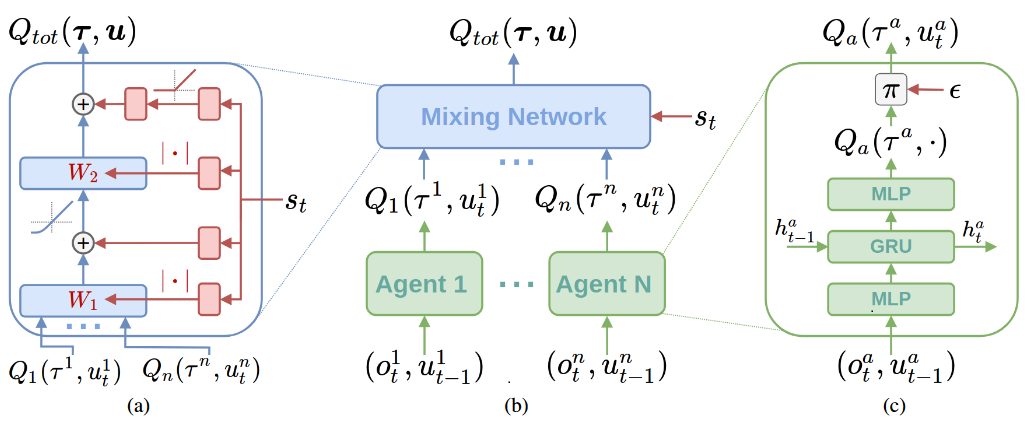
\includegraphics[width=\linewidth]{images/qmix.png}
  \caption{As presented in the QMIX paper: (a) Mixing network structure. In red are the hypernetworks that produce the weights and biases for mixing network layers showning blue. (b) The overall QMIX architecture. (c) Agent network structure. Best viewed in color}
  \label{fig:qmix}
\end{figure}

\subsection{Contributions to Reinforcement Learning}

Independent Q learning was one of the earliest attempts at multi-agent reinforcement learning and it's still the most commonly applied method for multi-agent learning. Two papers using a combination of IQL and Deep Q learning show strong results\citep{tampuu2017multiagent}\citep{leibo2017multi}. In IQL each agent has its own action-value function Q, however this approach does not clearly show the interactions between the agents. Multi-agent credit assignment is an interesting issue when it comes to decentralized cooperating agents. The approach taken by COMA is to take the existing reward function and remove the limitations while still being efficient.
QMIX takes another approach, $Q\textsubscript{tot}$ is the sum of all individual Q functions, one for each agent. But instead of using a simple sum, QMIX uses a monotic function.

\subsection{Future plans}
The next step for QMIX and COMA is to conduct additional tests with a larger number of agents. In COMAs case, centralized critics are harder to train and exploration becomes challenging. QMIX has plans to add more coordinated exploration schemes for settings with a larger number of learning agents. The SMAC environment is also planning on adding new challenging scenarios which require a high level of coordination between agents.

% Joep
\section{AlphaStar}
\label{chapter:alphastar}

\subsection{About}
The goal of DeepMind is to build general artificial intelligence (AI). In order to benchmark an AI system, it is critical to test the performance of the agent in diverse scenarios. Gaming environments have become an important tool to test the capabilities of an agent. They provide clear definitions for winning and losing, their strategies can often be translated to general problems and any action taken within this environment does not affect the real-world.

Since the foundation of DeepMind in 2010, they have created several AI systems that reached a superhuman level of play. In 2003, DeepMind presented their AI system that was able to exceed all previous AI based approaches on six out of seven Atari 2600 games and outperformed a human expert on three of them \citep{mnih2013playing}. In March 2016, DeepMind’s AlphaGo won a game of Go against grandmaster Lee Sedol \citep{borowiec2016alphago}. 

The next step for DeepMind was to build an AI system for a more complex environment, StarCraft II. In cooperation with Blizzard Entertainment, DeepMind introduced the StarCraft II learning environment (SC2LE) \citep{vinyals2017starcraft}. Together with this environment, DeepMind has created a baseline agent and tested its results on several mini-games. However, the most interesting problem for them was to create an agent capable of playing a full competitive game of StarCraft II. This agent was named AlphaStar.

The official peer-reviewed paper regarding AlphaStar is not yet published. The information in this chapter is based DeepMind's blog post \citep{alphastarblog} and the papers it refers to. 

\subsection{Applied Methods and Techniques}
The applied methods and techniques in this section are categorized into the architecture and the training of AlphaStar. Because the official paper has not been released yet, any information about the motivation of the applied methods and techniques regarding AlphaStar is hypothetical. 

\subsubsection{The architecture of AlphaStar}~\\ 

As the authors of the blog post state: "AlphaStar's neural network architecture applies a transformer torso to the units \citep{vaswani2017attention}, combined with a deep LSTM core \citep{hochreiter1997long}, an auto-regressive policy head \citep{vinyals2017starcraft} with a pointer network \citep{vinyals2015pointer}, and a centralized value baseline \citep{alphastarblog}."

The transformer torso \citep{vaswani2017attention} is a sequence transduction model based solely on attention mechanisms. Traditional neural network architectures for solving sequence to sequence problems are based on recurrent layers. A critical constraint of this recurrent model is that it precludes parallelization since each layer conditions on the output of its previous layer. Another downside of this layer-per-layer approach is that the decoding layers have to travel across the whole network to access the first encoder's hidden state. The larger the path length, the more difficult it becomes to learn long-range dependencies \citep{hochreiter2001gradient}. The attention mechanisms in the Transformer allow the decoding layers to attend over every input layer directly. This method reduces the path length to a constant number and additionally allows parallelization. A game of StarCraft involves thousands of actions in which an early action's influence might only be noticeable  much later in the game, using a transformer makes it easier to learn these long-range dependencies. 

A pointer network \citep{vinyals2015pointer} is a neural architecture that allows the size of the output dictionary to be variable depending on the size of the input dictionary. The sequence-to-sequence \citep{sutskever2014sequence} and the input-attention model \citep{bahdanau2014neural} were used to form the baseline for this pointer network. The issue with these baseline models is that they require a fixed output size. The introduced pointer network solves this issue by using attention as a pointer to select a member of the input sequence as the output.

\subsubsection{The training of AlphaStar}~\\

The training of AlphaStar can be split into two stages. During the first stage AlphaStar’s neural network was trained by imitation learning from replays of human games. From these replays, AlphaStar was able to learn the basics of micro- and macromanagement strategies. This first version was able to beat the built-in “Elite” AI in 95\% of the games. In the second stage the DeepMind team used this first version to seed a multi-agent league in which a reinforcement learning process was applied. In each iteration of this league, new competitors were added by branching from existing competitors. These new agents typically play against competitors in proportion to the opponents win-rate. This prevents catastrophic forgetting, since the new agent must be able to beat all previous versions of itself. To discover unlikely strategies, DeepMind included a policy distillation cost to ensure that the agent continues to try human like behaviors with some probability. To encourage the agents to learn specialized strategies, each agent is given its own learning objective. The neural network weights of this agent are then updated by applying  reinforcement learning, to optimize its own learning objective. The authors of the AlphaStar blog describe this weight update rule as follows: 
"The weight update rule is an efficient and novel off-policy actor-critic \citep{espeholt2018impala} reinforcement learning algorithm with experience replay \citep{lin1992self}, self-imitation learning \citep{oh2018self} and policy distillation \citep{rusu2015policy}".

\subsection{Contributions to Reinforcement Learning}
AlphaStar is the first AI system that beat a professional human player in a RTS game. In December 2018 DeepMind invited teams Liquid's TLO and MaNa, two professional StarCraft players, to play against their AlphaStar in a Protoss versus Protoss matchup. AlphaStar won both matchups in a 5-0 series. Interesting to note is that AlphaStar used different strategies to win these games and some of these strategies were considered sub-optimal by pro players.

A point of criticism in terms of fairness in these games was that AlphaStar was able to see the entire map at once, while a human player has to move its camera to view specific areas. To address this, DeepMind trained a whole new agent that did not have this advantage. This new agent was put up against MaNa for a second time. In this game, MaNa actually copied one of the strategies AlphaStar used to beat him before. So while the initial version of AlphaStar was learning from human play, its final version was teaching professional players new strategies. However, MaNa was able find a weakness in this the newly created agent and exploited this weakness to win the game, making the total score of AlphaStar against professional players 10 to 1.

\subsection{Future plans}

The advanced neural network architecture of AlphaStar has proven to be capable of reaching a superhuman level of StarCraft II gameplay. To reach this level of play, AlphaStar heavily relied on the possibility for agents to play against each other in the AlphaStar league and evolve during the process. We think that it would be valuable to do more research on how this technique can be applied to real-world applications that do not have clear winning conditions, such as weather prediction. An interesting research question would be to explore the possibility of letting two weather prediction agents 'battle' against each other and determine the better agent. 

\section{Conclusion}
% Real-Time Strategy games have been around for a very long time. However, the elements of RTS games have not changed much over the last years. Gathering resources, building units and buildings and scouting the environment to ultimately defeat the opponent have been the main goals of most RTS games. All these tasks combined can be very complex and has been proven an interesting field of research for Artificial Intelligence.

This paper has presented why RTS games are currently seen as a new horizon for AI research and has delved into a selection of state-of-the-art AI algorithms, hopefully providing a good starting point to those who wish to learn more about this research field.


% Misschien is dit juist wel allemaal nice voor in de intro/voor de research question
% A lot of research has already been done on certain topics in RTS games. Most of that research is focused on one or more tasks like planning, producing units or micromanagement. Often, different research on the same task proposes a different approach, which in turn delivers different performance. Because there already has been a lot of research on a lot of different tasks, a selection has been made from all of the research papers that have been surveyed. The selection has been made based on a variety of promising techniques applied to different tasks in RTS games, to cover a lot of topics. The purpose of this literature survey is to give the reader a notion of different Artificial Intelligence techniques that can be used to train agents that execute specific tasks in Real-Time Strategy games. 

Of all the algorithm reviews, the first technique is the learning of macromanagement based on live-action replays. This technique uses a neural network which is trained to predict the next build  on a given game state. The advantage of this, is that training times can be improved enormously. However, the performance is always related to the quality of the training data. 

The second technique is the use of a Genetic Algorithm to optimize building placement. The Genetic Algorithm tries to find the optimal building placement which can turn an attack on the base from a major loss into a win. \textbf{Add advantages and disadvantages.}

Another promising technique is the use of a Relational Markov Decision Process framework to generalize plans in different environments. \textbf{Add advantages and disadvantages.}
% Werking en positieve/negatieve punten toevoegen

Next, a paper is discussed which uses multiple AI techniques in a specific testing environment: MultiStar. Here, the performance of different reinforcement learning agents is tested against each other. The different techniques that are used are COMA and QMIX. \textbf{Add advantages and disadvantages.}
% Werking en positieve/negatieve punten toevoegen

Finally, AlphaStar is discussed, which is an AI system capable of beating professional players in a competitive StarCraft game. The neural network of AlphaStar applies an advanced architecture that is  capable of long-range sequence transduction with limited knowledge of the state. However, the training of this network relied on clear winning conditions between agents.

% Nog iets om het af  te maken?
At the end of this long research journey, it has become apparent that there are many different and unique algorithms which try to solve the distinct challenges presented by RTS games. Those that have been discussed in this review give a broad idea how creative the research community is and shows that AI is still very much an open-ended question.

\section{Acknowledgements}
We would like to thank our supervisor, Aleksander Czechowski, for his guidance, valuable feedback and support.

\onecolumn
\begin{appendices}
%   \section{General overview of RTS algorithms}
%   \begin{appendixfig}
%     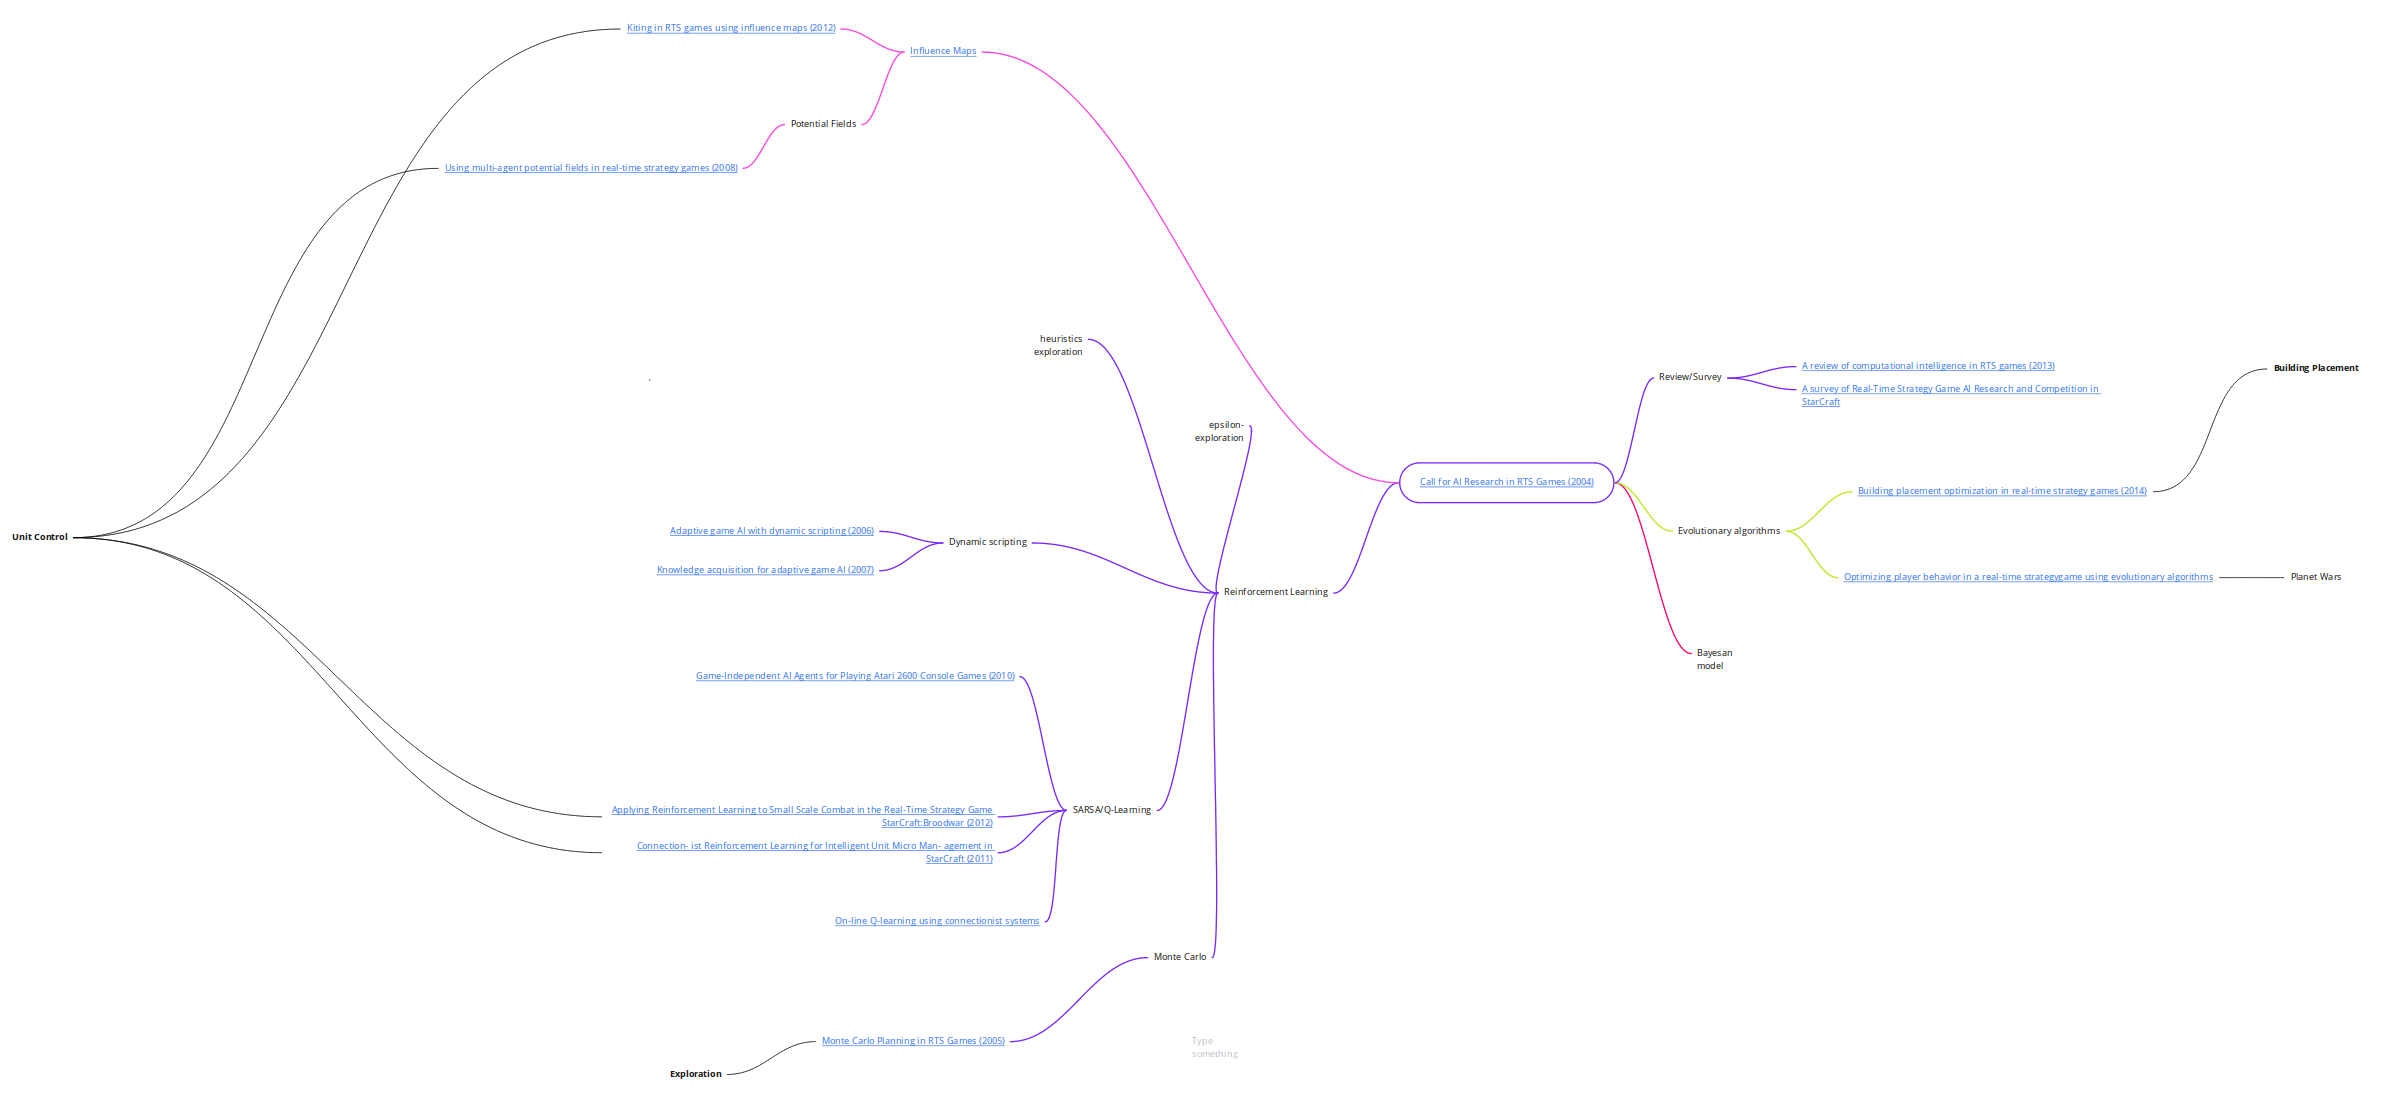
\includegraphics[width=\textwidth, angle=90, origin=c]{images/mindmap.png}
%     \label{}
%   \end{appendixfig}
%    \begin{sidewaysfigure}[h]
%    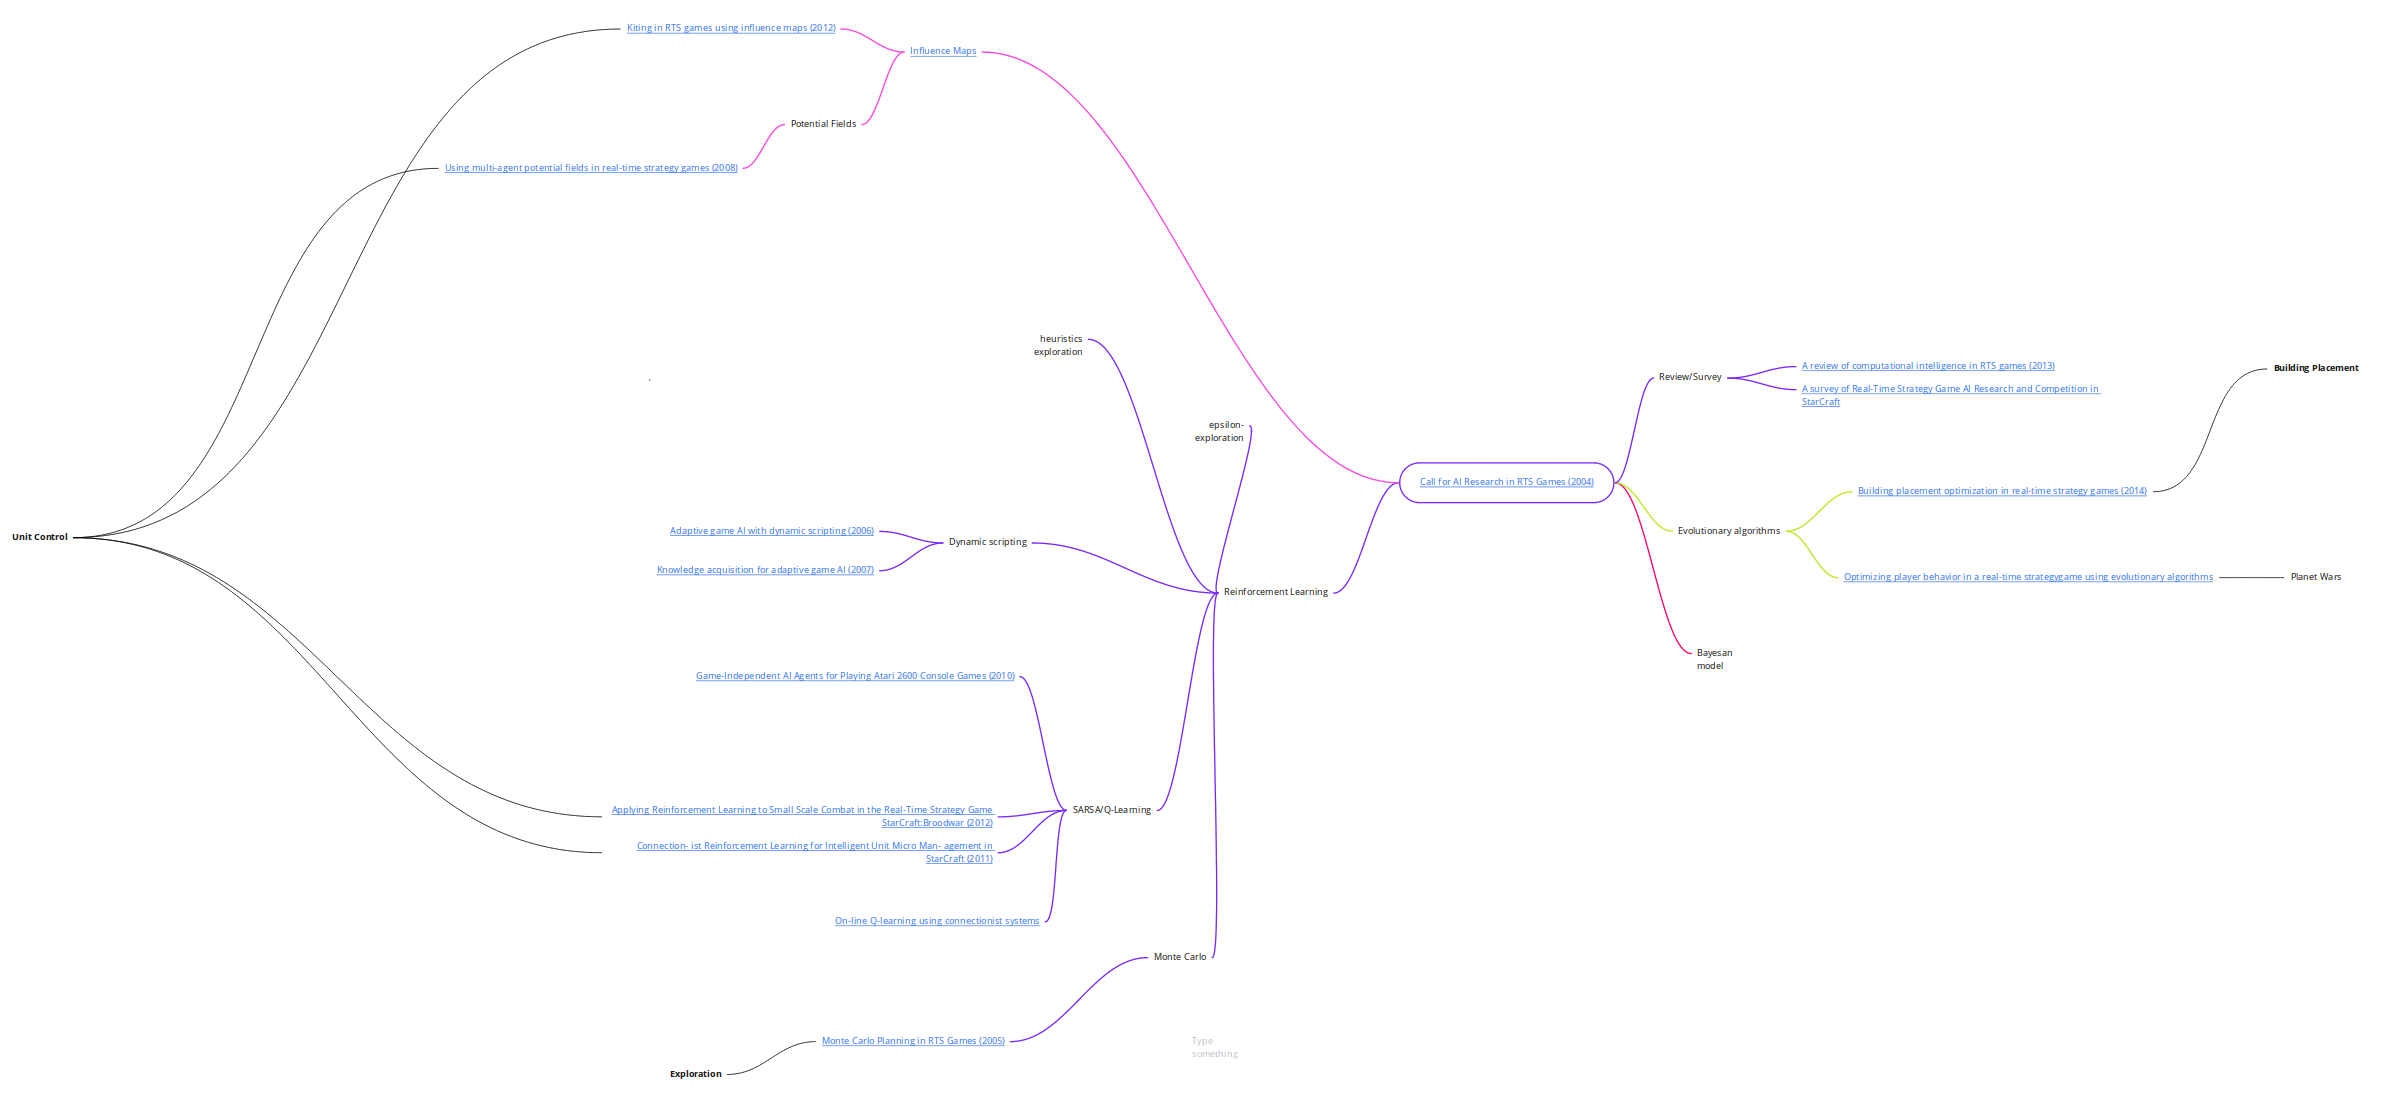
\includegraphics[width=0.5\textwidth, keepaspectratio]{images/mindmap.png}
%    % \caption{Property profile of the diverse library compared to the compound pool.}
%    \label{fig:PropProf}
%    \end{sidewaysfigure}
    \newpage
    \section{What is a Markov decision process?}
    \label{chapter:mdp}

\subsection{Basic idea behind the model}
People consider multiple times a day what actions they should and could take at a given moment. Before picking an action to perform the effects following the actions should be contemplated, these effects will be called rewards. Picking between actions with immediate rewards is easy because you can just pick the one with the best reward. But what if an action has a bad immediate reward but a better long term one. So the right arrangement between immediate rewards and future rewards has to be made.
\subsection{A standard Markov Decision Process}
With this idea in mind a Markov Decision Process (MDP) is created using four components:
\begin{enumerate}[nolistsep]
\item ${\displaystyle S}$ is a finite set of states
\item ${\displaystyle A}$ is a finite set of actions
\item ${\displaystyle P}$ is the effect the actions have on the state
\item ${\displaystyle R}$ is the immediate value of the actions
\end{enumerate}
\par
The state is the environment in which the agent operates, the actions the agent chooses to execute will transform the environment. A set of states is every possible variation the environment could be, each of these states would be a state in the MDP. The actions that are available to the agent depend on the scenario it is in, for example, the action \textit{open the door} would only be available if the agent is in a scenario where a door is available to be opened. For every scenario the agent is in, it has a set of possible actions it could pick from. The transition specifies how each actions modifies the state, this is something to consider when deciding between actions. The MDP will learn a policy, the policy specifies the best action to take for each of the states.
\subsection{Partial Observable Markov Decision Process}
The standard MDP is designed for an scenario where an agent has an complete view of the environment, however this is often not the case for a real world scenario where an agent has a scarce view of the environment. Performing actions on local observations and nothing more is desired in a scenario like this. Making an action based on the whole current state presents no problem when you have an complete view of the environment. But an partial view of the environment clouds the idea of the current state and what it looks like. To satisfy these new demands modifications were needed to the standard MDP. A Partial Observable Markov Decision Process (POMDP) was created with the same four component as a standard MDP, the only difference is whether or not the current state is observable. A new component was added:  ${\displaystyle \Omega}$ is a set of observations. These observations are provided by the state and can be used to get a idea about the current state. These observations can be probabilistic; so an observation model needs to be created. This model tells the probability of each observation for each state in the model.
\par
With the added partial observability the model no longer has direct access to the current state, the decisions condition on the entire history of the process. So an extra component is added: ${\displaystyle O}$ is a set of conditional observation probabilities. Instead of keeping track of the starting situation, all actions performed and all observations seen; the same information can be extracted from the probability distribution over all the states. 
\subsection{Decentralized partially observable Markov decision process}
What if there are two agents which a scare view of the environment. In the current model of POMDP the agents see each other as part of the state. To solve this multi-agent problem a new model was created called \textit{Decentralized partially observable Markov decision process} (Dec-POMDP). Instead of tracking the actions and observations of an individual agent, the joint actions and observations of all agents will be tracked. In a Dec-POMDP agents only know their own individual action and do not observe the actions of the other agents. Each agent acts on their own individual observations and no additional communication is assumed. The agents can however communicate through the state, if an agent needs to modify a property of the state the other agents will get the updated version of the state. In a Dec-POMDP at each stage each agent takes an action and receives local observations and a joint immediate reward. The observations they receive are individual observations but the reward generated by the environment is the same for all agents. The policy in a standard MDP specifies what the best action to take is, but since there are multiple agents who each have to take actions based on their own local observation; A local and joint policy is created.

\end{appendices}
\twocolumn

% \onecolumn
% \appendix
% \chapter{General overview of algorithms used for RTS games}
% \begin{sidewaysfigure}[t]
%     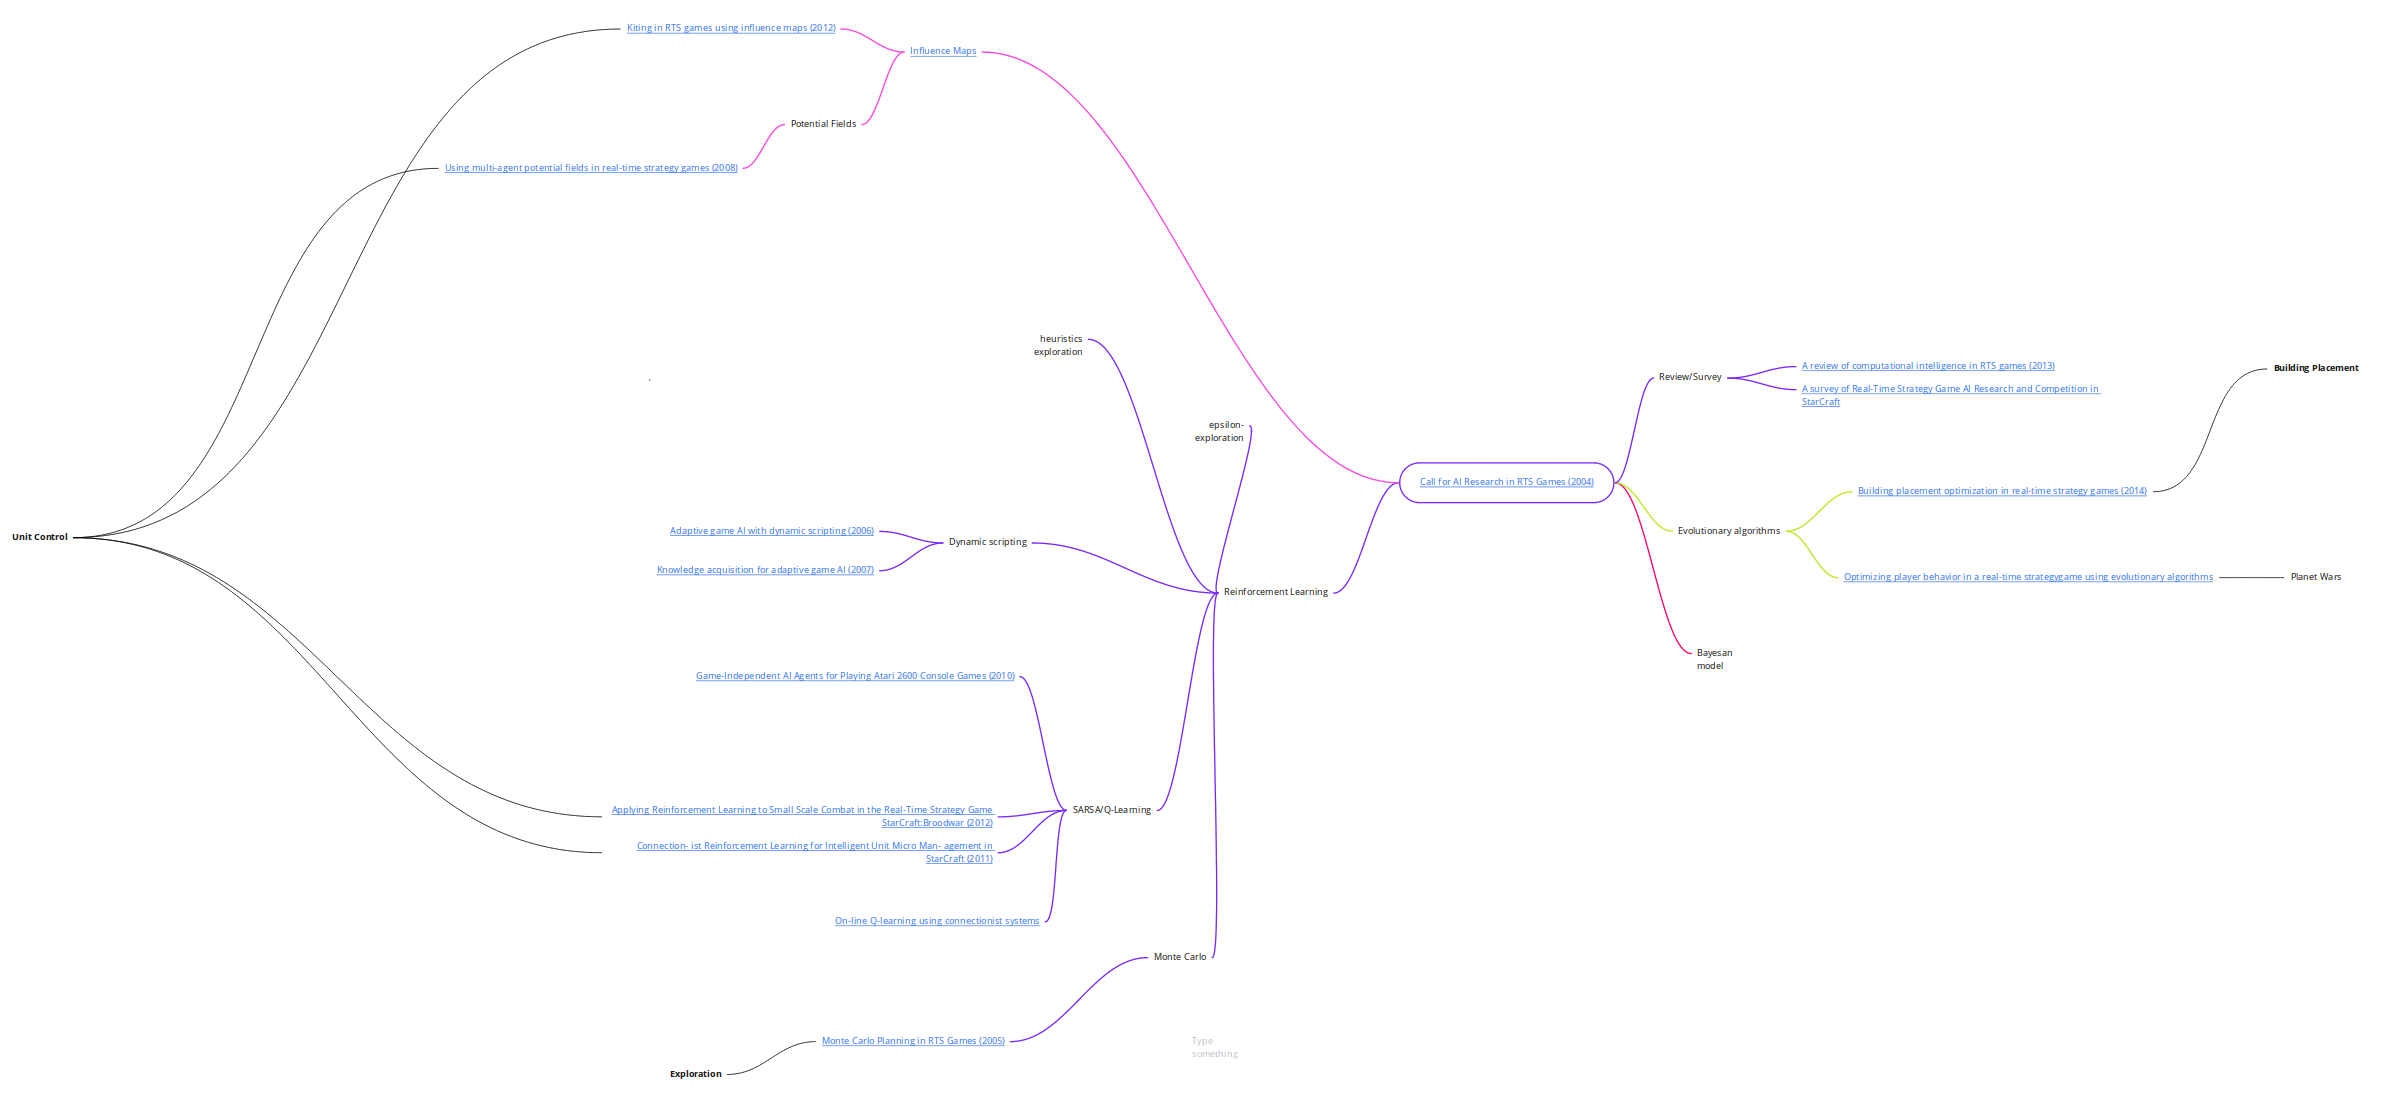
\includegraphics[width=\textwidth,height=\textheight,keepaspectratio]{images/mindmap.png}
%     % \caption{Property profile of the diverse library compared to the compound pool.}
%     \label{fig:PropProf}
% \end{sidewaysfigure}
% \twocolumn

\bibliographystyle{unsrt}
\bibliography{references}
\end{document}
